\begin{frame}{LaMa: Large Holes Need a Global Receptive Field}
  \begin{center}
    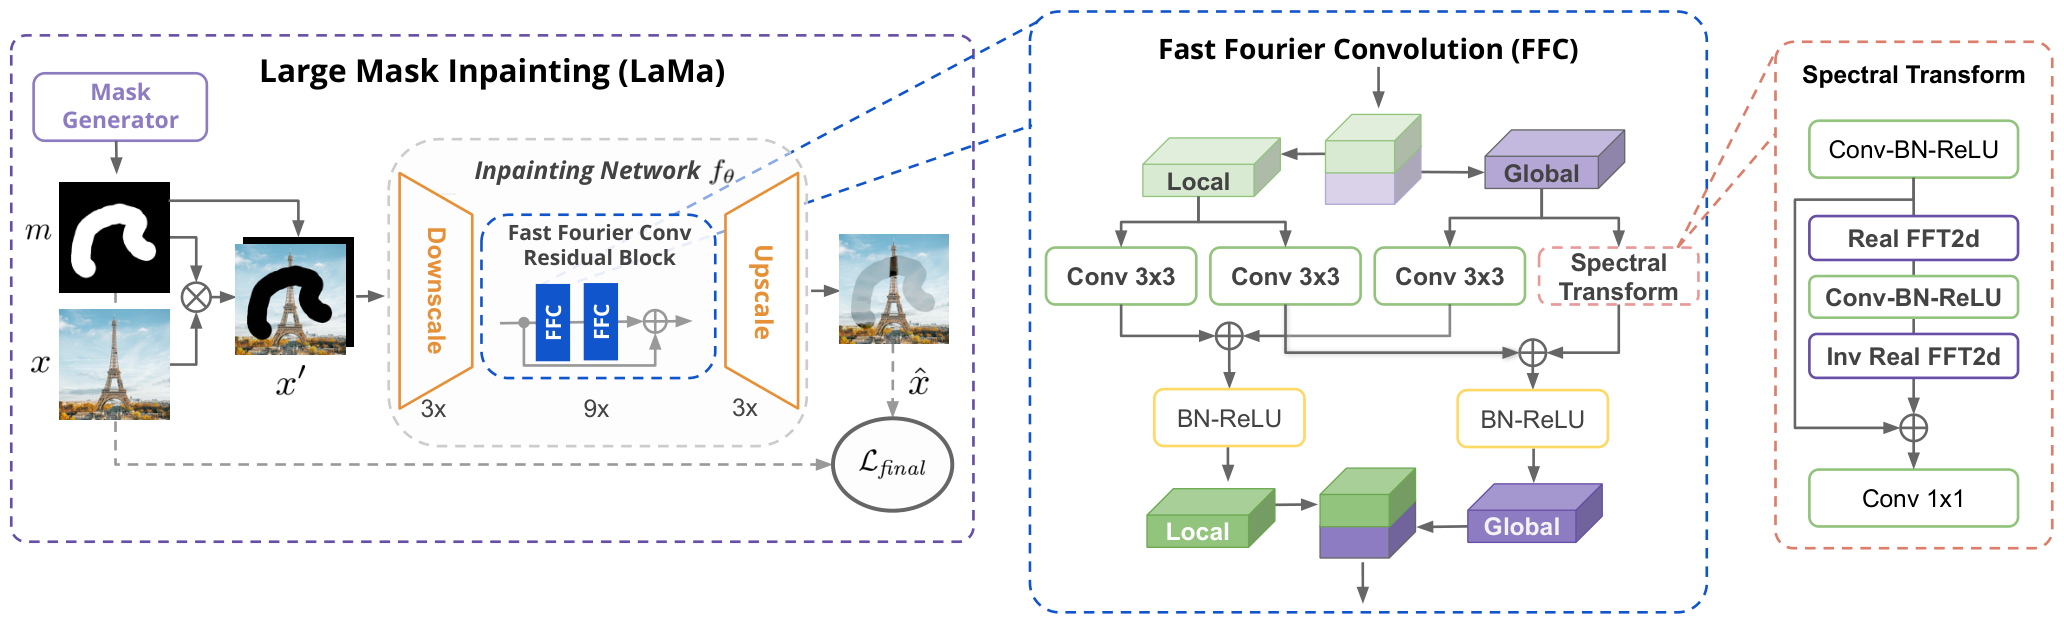
\includegraphics[width=\textwidth,height=0.34\textheight,keepaspectratio]{images/image-restoration-applications/lama_fig2_architecture.png}\\[0.2em]
    {\scriptsize Suvorov et al., ``Resolution-robust Large Mask Inpainting with Fourier Convolutions,'' WACV 2022, \href{https://arxiv.org/abs/2109.07161v2}{arXiv:2109.07161v2}, Figure~2.\par}
  \end{center}
  \vspace{-0.6em}
  \begin{itemize}\footnotesize\itemsep0.3em
    \item \textbf{Inpainting} fills a masked region so that it agrees with the rest of the image; masks range from thin scribbles to large boxes and whole objects.
    \item \textbf{LaMa} traces failures on large holes to a receptive field that is too small, in the network and in the loss. Three fixes: (i) fast Fourier convolutions (FFC), whose global branch convolves in the frequency domain (real FFT, convolution, inverse FFT), so even early layers see the whole image; (ii) a perceptual loss computed with a high-receptive-field segmentation network; (iii) training on wide and large masks.
    \item Trained only at $256 \times 256$, it generalises to much higher resolutions and continues periodic structure such as bricks and windows. It has 27M parameters (Big LaMa: 51M, trained on 4.5M Places images) and needs one forward pass per image.
  \end{itemize}
\end{frame}

\begin{frame}{Conditioning a Diffusion Model on a Mask}
  \begin{columns}[T,onlytextwidth]
    \column{0.56\textwidth}
      \begin{itemize}\footnotesize\itemsep0.25em
        \item \textbf{Trained conditioning.} The SD~1.5 inpainting checkpoint adds 5 U-Net input channels, 4 for the masked image's VAE latent and 1 for the mask, zero-initialised and fine-tuned for 440k steps.
        \item \textbf{Training-free: RePaint} (CVPR 2022) keeps an unconditional diffusion model and, at every reverse step, pastes in the known pixels noised to the current level:
        \[ x_{t-1} = m \odot x^{\text{known}}_{t-1} + (1 - m) \odot x^{\text{gen}}_{t-1}, \]
        with $m = 1$ on known pixels, $x^{\text{known}}_{t-1} \sim q(x_{t-1} \mid x_0)$ from the forward process and $x^{\text{gen}}_{t-1} \sim p_\theta(x_{t-1} \mid x_t)$ from the model.
        \item \textbf{Resampling.} Pasting alone matches texture but not meaning, so RePaint re-noises $x_{t-1}$ to $x_t$ and denoises again several times: any mask works without retraining, at the cost of extra network evaluations.
        \item Pasting is a projection, exact only for noiseless measurements; DPS takes a gradient step instead.
      \end{itemize}
    \column{0.42\textwidth}
      \centering
      \vspace{0.6em}
      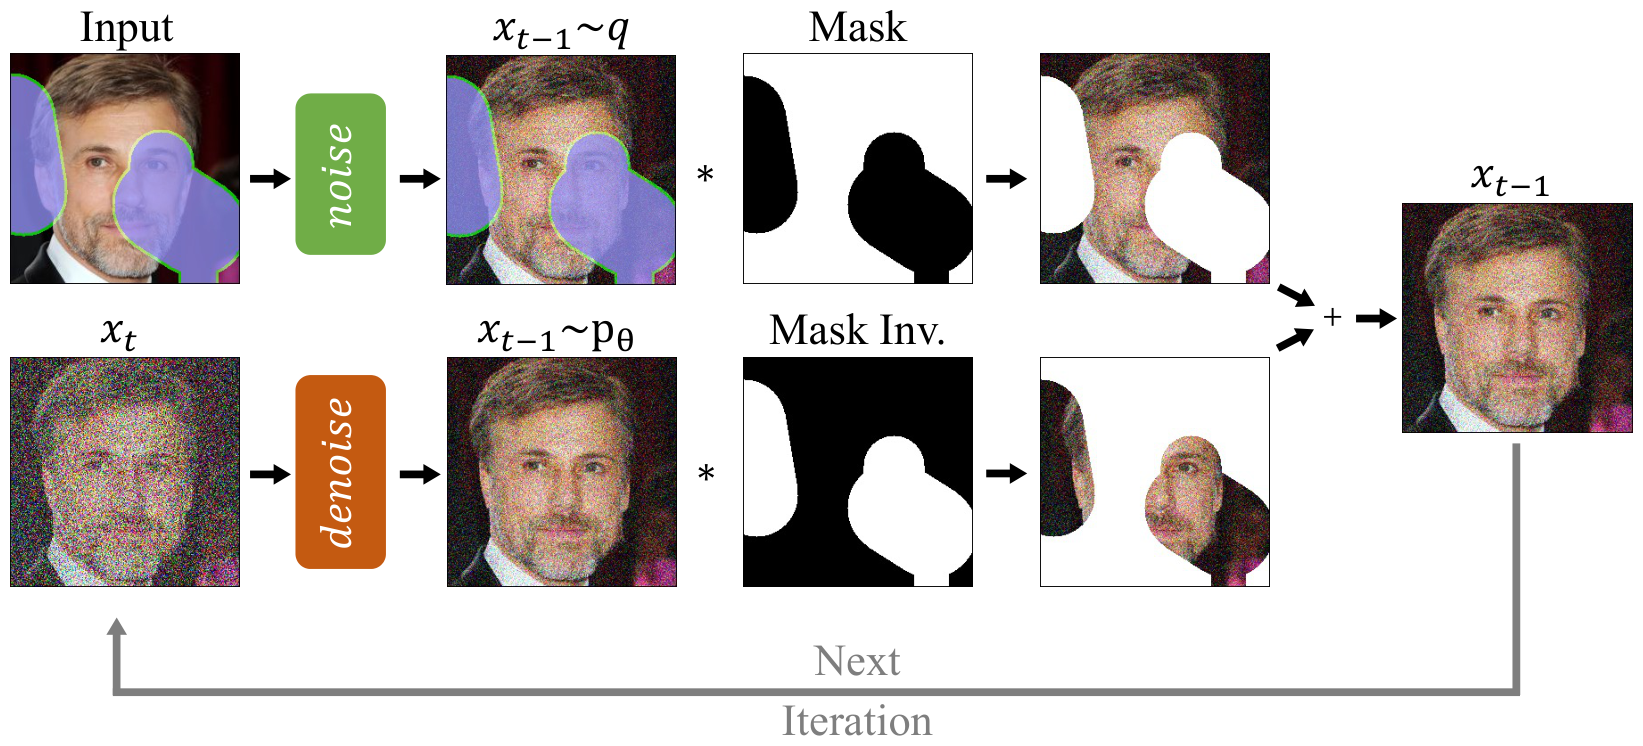
\includegraphics[width=\linewidth,height=0.46\textheight,keepaspectratio]{images/image-restoration-applications/repaint_fig2_overview.png}\\[0.2em]
      {\scriptsize Top: known region from the noised input; bottom: model sample for the hole. Lugmayr et al., ``RePaint: Inpainting using Denoising Diffusion Probabilistic Models,'' CVPR 2022, \href{https://arxiv.org/abs/2201.09865v4}{arXiv:2201.09865v4}, Figure~2.\par}
  \end{columns}
  {\scriptsize SD~1.5 inpainting \href{https://huggingface.co/stable-diffusion-v1-5/stable-diffusion-inpainting}{model card}.\par}
\end{frame}

\begin{frame}{Plug-In Inpainting for Any Base Model}
  \begin{columns}[T,onlytextwidth]
    \column{0.52\textwidth}
      \begin{itemize}\footnotesize\itemsep0.25em
        \item \textbf{Dedicated models} (a) mix all inputs with the text from the first layer, so text can drown out image evidence; each new base model needs a new fine-tune.
        \item \textbf{BrushNet} (ECCV 2024, c): a trainable U-Net copy without cross-attention reads the noisy latent, masked-image latent and mask, and adds its features to the frozen base through zero convolutions; the known region is pasted back through a blurred mask. Community fine-tunes keep working.
        \item \textbf{PowerPaint} (ECCV 2024) learns task prompts $P_{\text{obj}}$ (insert; box masks) and $P_{\text{ctxt}}$ (fill from context; random masks). For removal, classifier-free guidance takes $P_{\text{ctxt}}$ as positive and $P_{\text{obj}}$ as negative prompt.
        \item \textbf{FLUX.1 Fill} (Black Forest Labs, Nov.\ 2024): a 12B-parameter rectified-flow transformer that inpaints and outpaints from a mask and a prompt; the dev weights are non-commercial.
      \end{itemize}
    \column{0.46\textwidth}
      \centering
      \vspace{0.5em}
      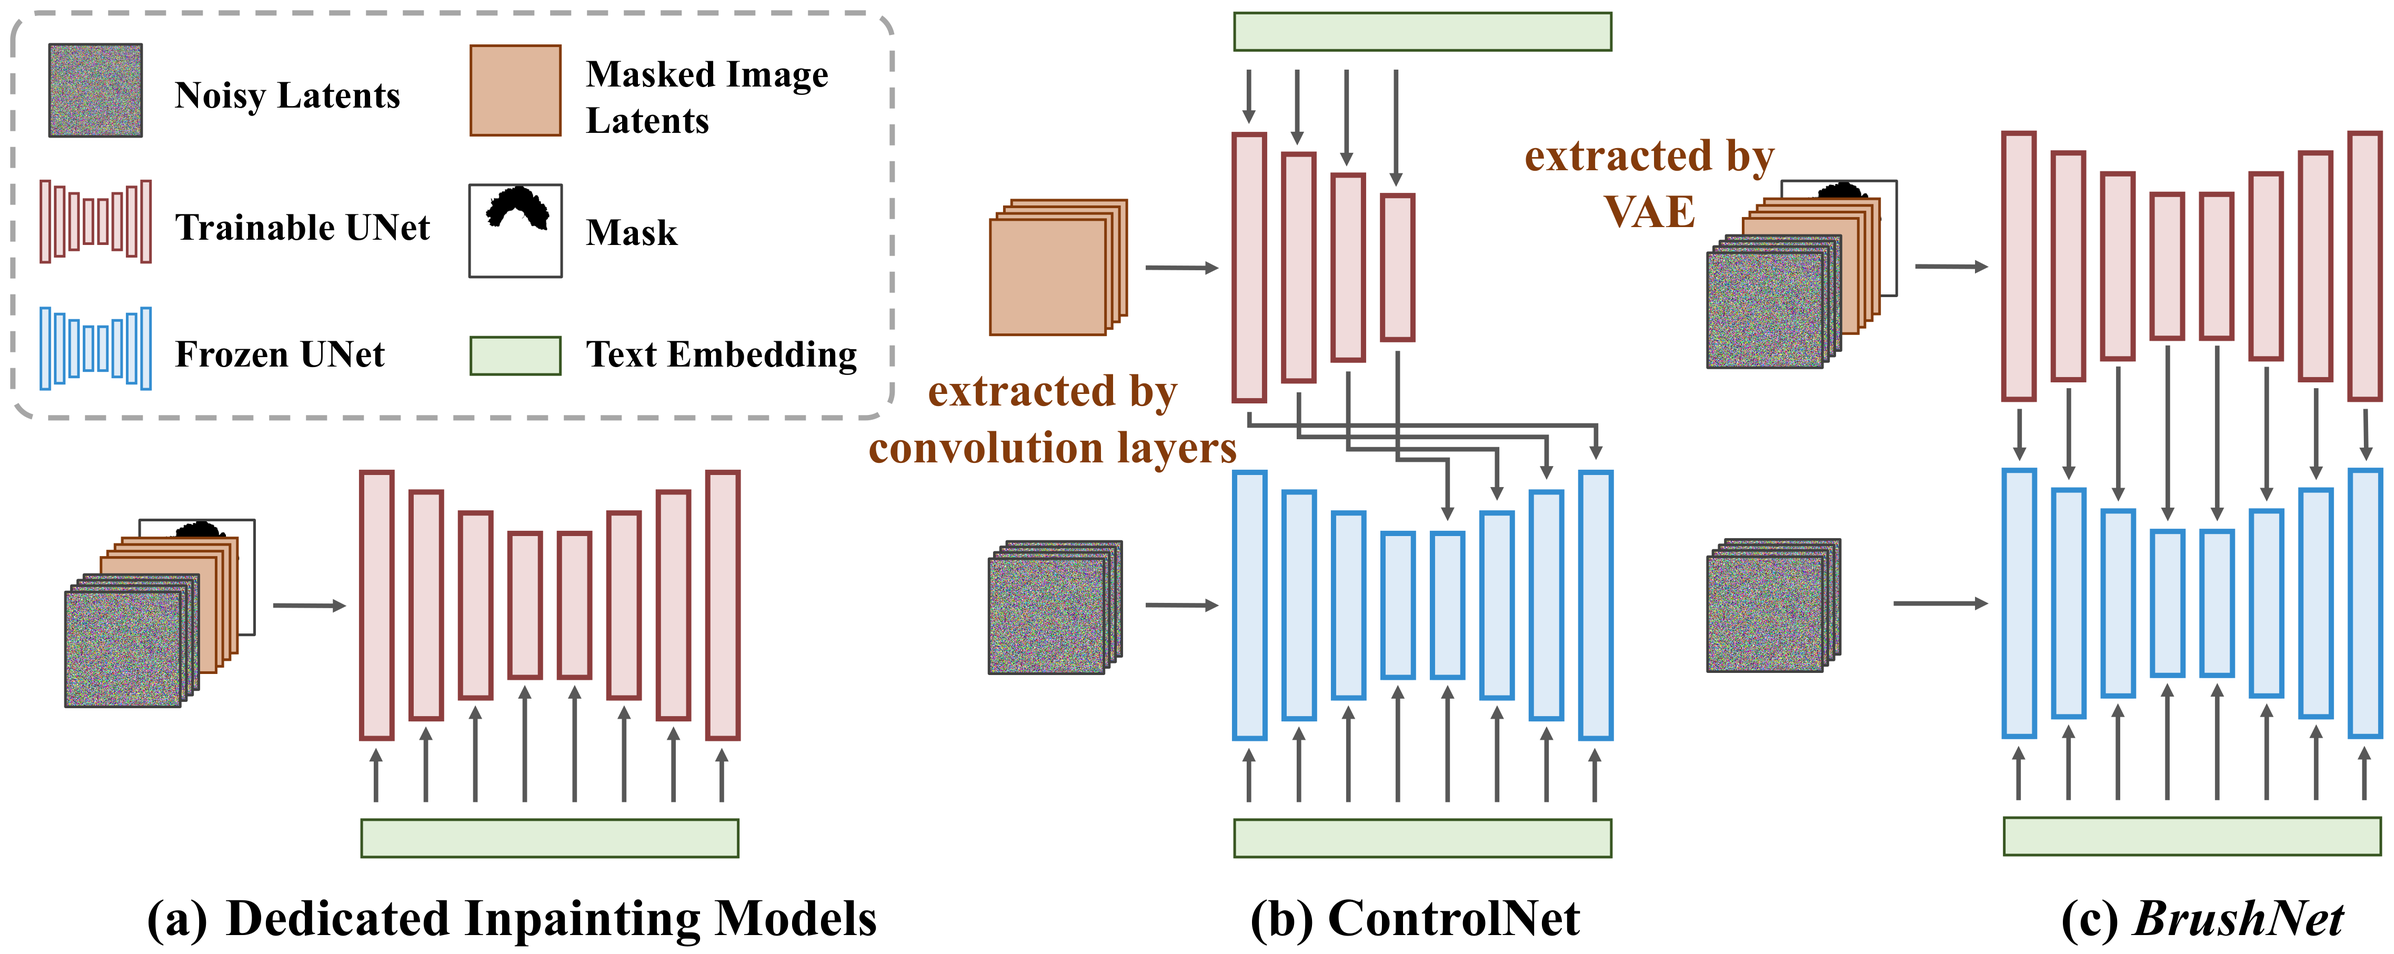
\includegraphics[width=\linewidth,height=0.38\textheight,keepaspectratio]{images/image-restoration-applications/brushnet_fig2_architectures.png}\\[0.2em]
      {\scriptsize Panel (b) is ControlNet. Ju et al., ``BrushNet: A Plug-and-Play Image Inpainting Model with Decomposed Dual-Branch Diffusion,'' ECCV 2024, \href{https://arxiv.org/abs/2403.06976v1}{arXiv:2403.06976v1}, Figure~2.\par}
  \end{columns}
  {\scriptsize Zhuang et al., ECCV 2024, \href{https://arxiv.org/abs/2312.03594v4}{arXiv:2312.03594v4}, Sec.~1 and 3; Black Forest Labs, ``Introducing FLUX.1 Tools,'' \href{https://bfl.ai/blog/24-11-21-tools}{bfl.ai/blog/24-11-21-tools}; \href{https://huggingface.co/black-forest-labs/FLUX.1-Fill-dev}{FLUX.1-Fill-dev model card}.\par}
\end{frame}

\begin{frame}{Object Removal Must Remove the Effects Too}
  \begin{columns}[T,onlytextwidth]
    \column{0.55\textwidth}
      \begin{itemize}\footnotesize\itemsep0.25em
        \item \textbf{Hole filling invents content.} A model trained to refill random holes tends to put a new object there; a tight mask leaves shadows and reflections behind (right).
        \item \textbf{ObjectDrop} (ECCV 2024): 2,500 tripod-shot counterfactual pairs, before and after physically removing one object; a diffusion model fine-tuned on them removes objects with their shadows and reflections.
        \item \textbf{2025 data engines.} OmniEraser mines over 100,000 object/background pairs from video; RORem grows 60K pairs to over 200K by human-in-the-loop filtering (success 7.6\% for the base model, 76.2\% after), and a 4-step variant (74.8\%) runs in under 1\,s; SmartEraser trains on over a million synthetic pairs, keeping the object visible as guidance.
        \item \textbf{No ground truth inside the mask.} PROVE (ACM MM 2026): full-reference metrics reward copy-paste and no-reference metrics favour blur, so it scores coherence between the filled region and its background.
      \end{itemize}
    \column{0.43\textwidth}
      \centering
      \vspace{0.4em}
      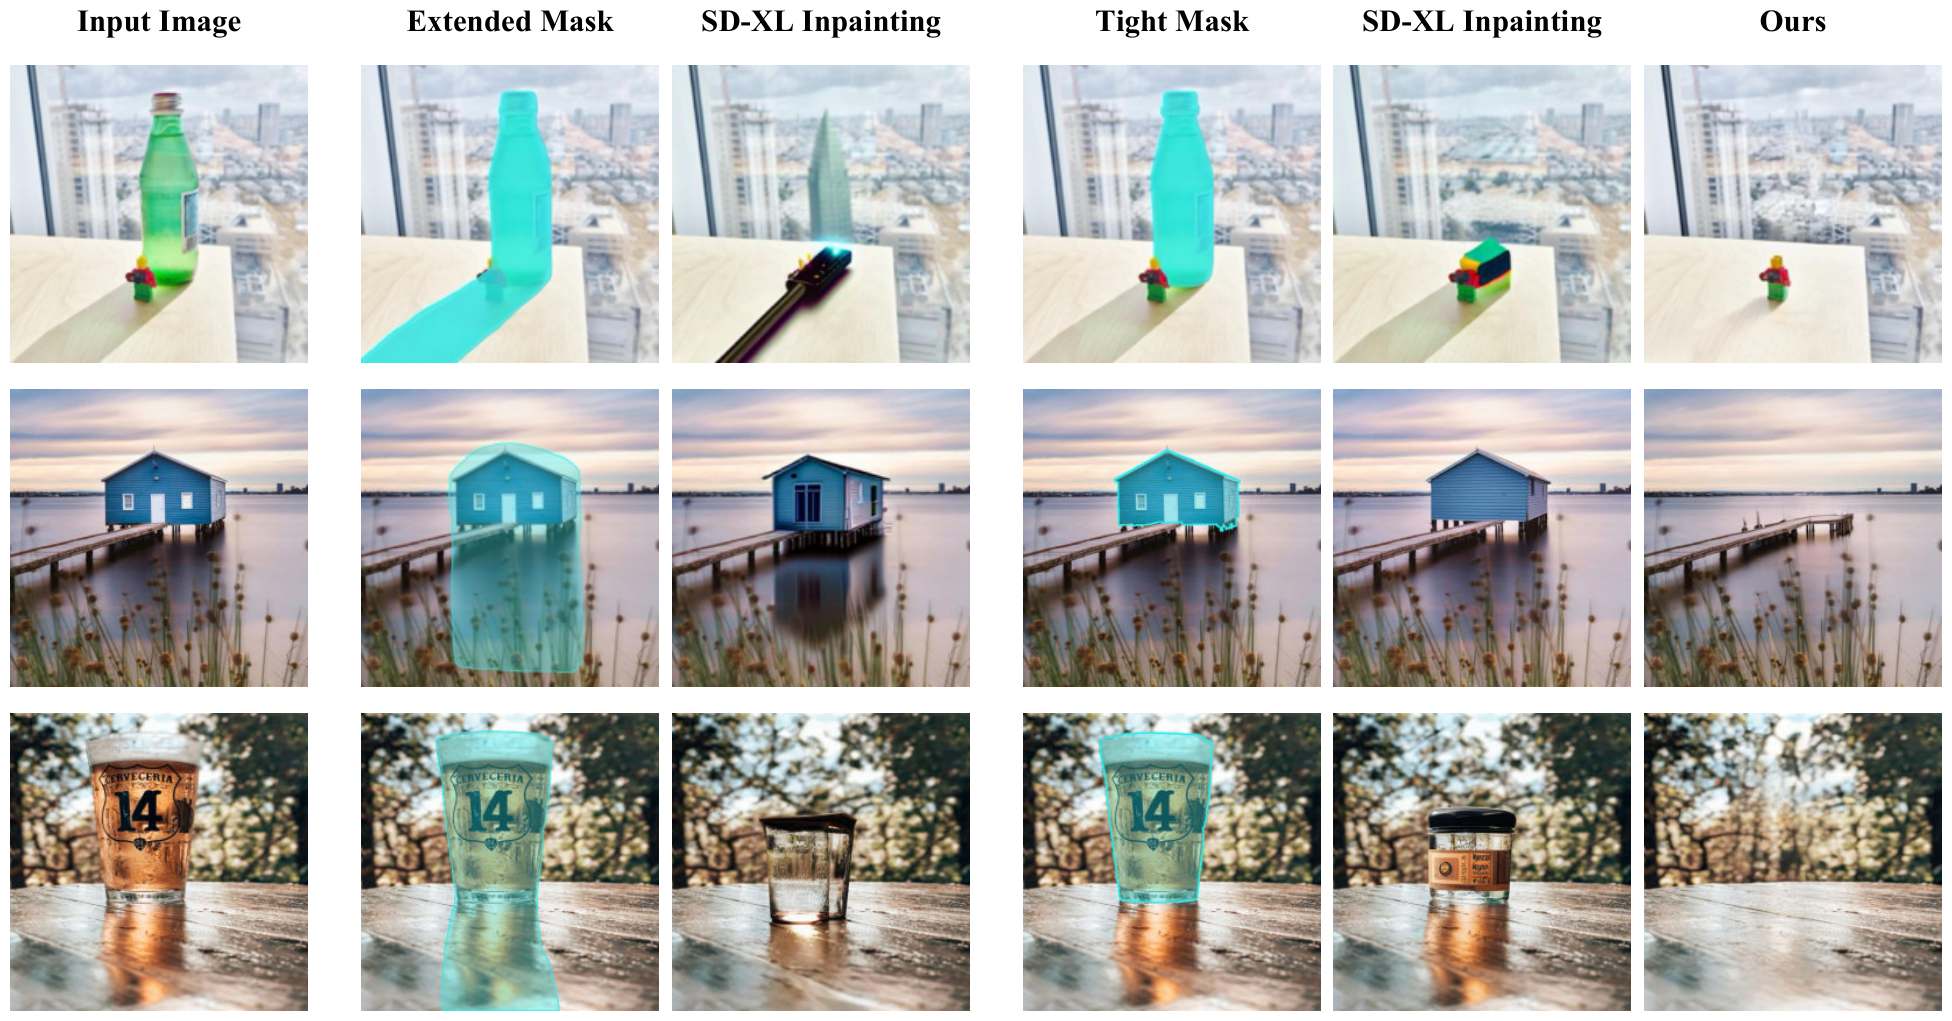
\includegraphics[width=\linewidth,height=0.38\textheight,keepaspectratio]{images/image-restoration-applications/objectdrop_fig4_removal_vs_inpainting.png}\\[0.2em]
      {\scriptsize SD-XL inpainting with an extended or a tight mask, versus ObjectDrop. Winter et al., ``ObjectDrop: Bootstrapping Counterfactuals for Photorealistic Object Removal and Insertion,'' ECCV 2024, \href{https://arxiv.org/abs/2403.18818v1}{arXiv:2403.18818v1}, Figure~4.\par}
  \end{columns}
  {\scriptsize OmniEraser: \href{https://arxiv.org/abs/2501.07397v3}{arXiv:2501.07397v3}; RORem: \href{https://arxiv.org/abs/2501.00740v3}{arXiv:2501.00740v3}, Sec.~4; SmartEraser: \href{https://arxiv.org/abs/2501.08279v3}{arXiv:2501.08279v3}; PROVE: \href{https://arxiv.org/abs/2605.14534v2}{arXiv:2605.14534v2}.\par}
\end{frame}

\begin{frame}{Removing Objects from Video}
  \begin{center}
    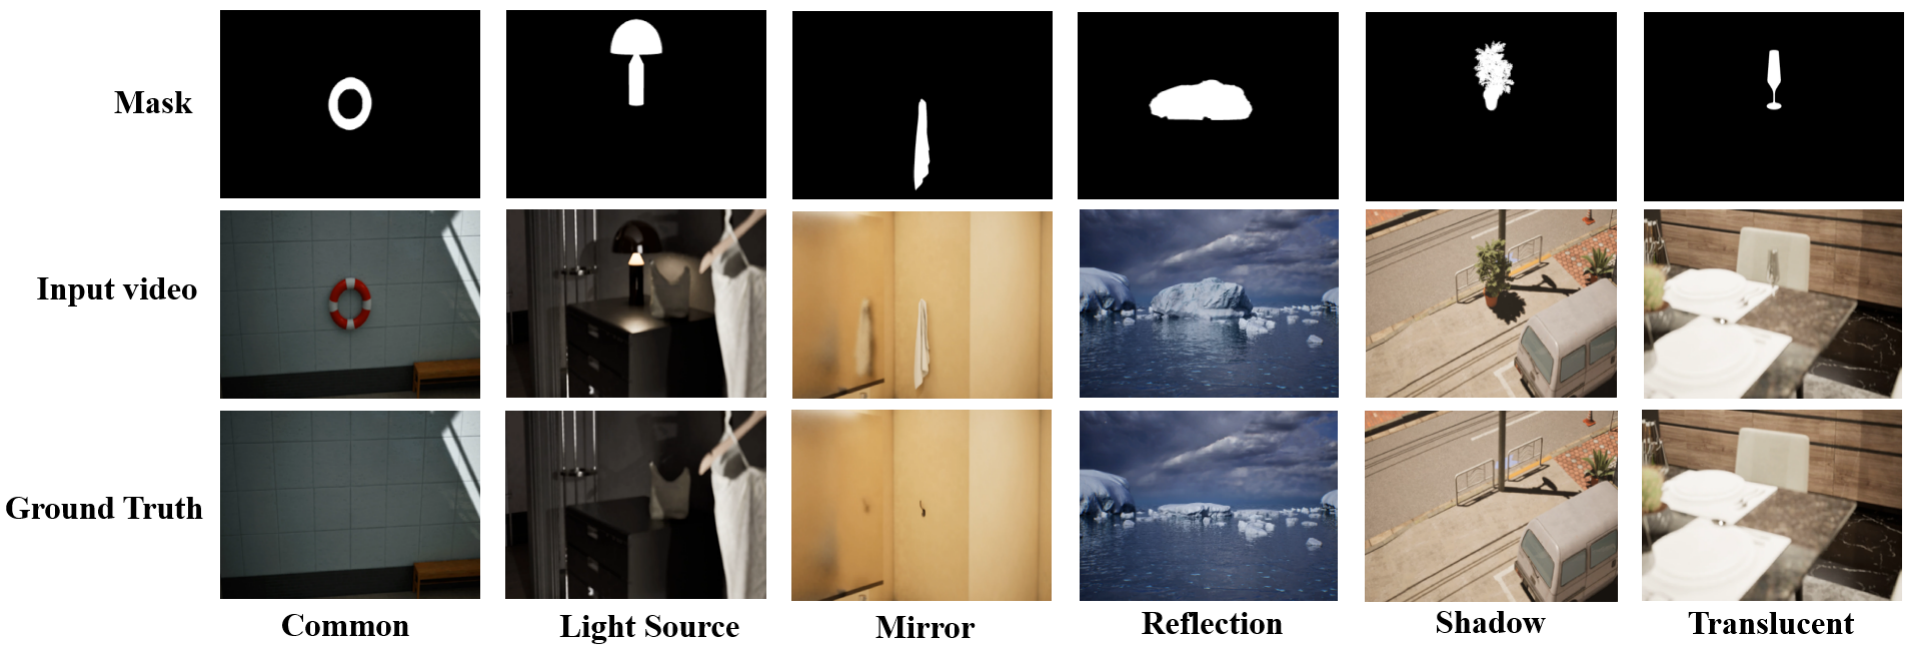
\includegraphics[width=\textwidth,height=0.25\textheight,keepaspectratio]{images/image-restoration-applications/rose_fig3_side_effects.png}\\[0.2em]
    {\scriptsize Rendered training pairs for six cases (mask, input, ground truth). Miao et al., ``ROSE: Remove Objects with Side Effects in Videos,'' NeurIPS 2025, \href{https://arxiv.org/abs/2508.18633v1}{arXiv:2508.18633v1}, Figure~3.\par}
  \end{center}
  \vspace{-0.8em}
  \begin{itemize}\footnotesize\itemsep0.2em
    \item \textbf{ProPainter} (ICCV 2023) completes the optical flow inside the mask, propagates known pixels from other frames in image and feature space, and fills the rest with a sparse video transformer: +1.46\,dB PSNR over prior methods.
    \item \textbf{DiffuEraser} (2025) adds a motion module to BrushNet and starts from ProPainter's output, inverted to noise with DDIM, to suppress hallucinated objects.
    \item \textbf{MiniMax-Remover} (NeurIPS 2025) strips text input and cross-attention from the Wan2.1-1.3B flow-matching video transformer and trains against adversarial ``bad'' input noise: 6 sampling steps, no classifier-free guidance.
    \item \textbf{ROSE} (NeurIPS 2025) also removes side effects (shadows, reflections, light, translucency, mirror images), learning from videos rendered with a 3D engine and predicting the affected area explicitly.
  \end{itemize}
  {\scriptsize Zhou et al., ICCV 2023, \href{https://arxiv.org/abs/2309.03897v1}{arXiv:2309.03897v1}; Li et al., 2025, \href{https://arxiv.org/abs/2501.10018v1}{arXiv:2501.10018v1}, Sec.~3; Zi et al., NeurIPS 2025, \href{https://arxiv.org/abs/2505.24873v1}{arXiv:2505.24873v1}.\par}
\end{frame}

\begin{frame}{Inpainting and Removal Models That Run Locally}
  Open checkpoints, with the licence stated in each official repository or model card (code licences; fine-tuned weights also carry their base model's terms):\\[0.4em]
  {\centering\scriptsize
  \begin{tabular}{>{\raggedright\arraybackslash}p{2.0cm} >{\raggedright\arraybackslash}p{2.1cm} >{\raggedright\arraybackslash}p{2.3cm} >{\raggedright\arraybackslash}p{2.0cm} >{\raggedright\arraybackslash}p{3.3cm}}
    \toprule
    \textbf{Model} & \textbf{Task} & \textbf{Size or base} & \textbf{Licence} & \textbf{Hardware notes from the source} \\
    \midrule
    LaMa (Big LaMa) & erase objects & 51M parameters & Apache-2.0 & IOPaint runs it on CPU, GPU or Apple Silicon \\
    PowerPaint & insert, remove, outpaint & SD 1.5 fine-tune & MIT & bundled in IOPaint \\
    BrushNet & text-guided inpainting & branch on a frozen SD U-Net & Apache-2.0 & plugs into community SD fine-tunes \\
    FLUX.1 Fill (dev) & inpaint, outpaint & 12B parameters & non-commercial & gated download \\
    RORem & remove objects & SDXL-inpainting fine-tune & Apache-2.0 (README) & 4-step variant: 0.50\,s at 512\,px, 0.83\,s at 1024\,px (A100) \\
    ProPainter & video inpainting & flow + transformer & S-Lab License, non-commercial & $720{\times}480$, 50 frames: 11\,GB (32-bit), 7\,GB (16-bit) \\
    DiffuEraser & video inpainting & SD + BrushNet & Apache-2.0 & ProPainter output as prior \\
    \bottomrule
  \end{tabular}\par}
  \vspace{0.4em}
  {\scriptsize IOPaint (Apache-2.0) is a self-hosted app serving LaMa, PowerPaint and BrushNet, \href{https://github.com/Sanster/IOPaint}{github.com/Sanster/IOPaint}. Licences and memory figures: official repositories and model cards, checked October 2026; RORem timings: Li et al., CVPR 2025, \href{https://arxiv.org/abs/2501.00740v3}{arXiv:2501.00740v3}, Sec.~3.4 and 4.2.\par}
\end{frame}
